\documentclass[]{article}
\RequirePackage{amsmath}

\usepackage{graphicx}
%\graphicspath{{./figures/}}
\usepackage{amssymb}
\usepackage{color}
\usepackage{hyperref}
\usepackage{algorithm}
\usepackage{algpseudocode}
\bibliographystyle{IEEEtran}
\newcommand{\knote}[1]{\textcolor{green}{A: {#1}}}
\newcommand{\dnote}[1]{\textcolor{red}{D: {#1}}}
\newcommand{\vk}[1]{\textcolor{blue}{V: {#1}}}
\newcommand{\lnote}[1]{\textcolor{cyan}{L: {#1}}}


\begin{document}
    \title{The Ergo Platform}

    \date{\today}
    \maketitle

    \begin{abstract}
        This document contains a general idea of Ergo platform and a high-level overview of it's main features.
        More details may be found in separate papers cited along this one.
    \end{abstract}

    \section{Vision}

    Ergo platform was started in 2017 after several years of research and prototypes implementations.
    Despite of huge hype around cryptocurrencies, the technology itself stuck close to it's initial stage.
    In pursuit of high profits and popularity, developers claimed an implementation of blockchain 2.0 (3.0 and so on),
    in prejudice of the main advantage of cryptocurrencies -- decentralization -- and promising that it will be achieved
    somewhere in the future.

    In opposite, the idea of Ergo is implement ready-to-use ideas keeping the network really decentralized.
    It may be called a blockchain 1.1 - a major update to the blockchain technology instead of
    a revolutionary breaking changes.
    The main focus of Ergo is to be the platform that is really useful for blockchain-demanded
    decentralized applications, and to be survivable in a long distance.
    Technical and economic solutions that will allow to achieve this will be described in the following sections.

    \section{Consensus}

    Consensus protocol of Ergo -- Autolykos -- is based on a well-known Proof-of-Work idea.
    PoW was chosen by several reasons: these protocols are widely studied, have high security guarantees
    and are friendly for clients since PoW validation is very fast. % and require minimal amount of data
    However, existing PoW protocols have known drawbacks: ASIC-equipped miners produce blocks
    orders of magnitude faster than regular miners, moreover
    they unite in mining pool and just few pool operators controls the network as a result.

    Autolykos is based on one list k-sum problem, that is similar to the known Equihash PoW~\cite{biryukov2017equihash}.
    Ergo uses Autolykos with parameters, that require from miners to keep 2 Gb of data in RAM,
    that reduces the advantage of ASICs over commodity hardware.
    Such memory-hard protocols are quite popular in cryptocurrencies, while the second property
    of Autolykos -- non-outsourcability -- is unique and to the best of our knowledge Ergo
    will be the first cryptocurrency that have it. Autolykos is constructed in such a way
    that if a mining pool outsources the puzzle to a miner, miner can recover pool's
    private key and steal the reward.
    This fact discourages formation of centralized pools and centralization of the
    network in the hands of pool operators, returning Ergo back to the original
    one-CPU-one-vote idea from the Bitcoin whitepaper.

    \section{Clients}

    For now, it is almost impossible to use cryptocurrencies without a help of trusted parties.
    Even if a client just want send some coins, he should download and process gigabytes of
    data to synchronize the network, which may take several weeks even on a high-end hardware,
    not to mention a mobile phones.
    No wonder that most of users prefer to use trusted solutions for wallets, exchanges, block
    explorers and so on.

    Ergo was designed to be maximally user-friendly in the sense of decentralization.
    One of important properties of PoW is that it allows to verify the work done without
    downloading the full chain.
    Ergo block headers supports NiPoPoW~\cite{kiayias2017non} proofs, allowing light clients
    to synchronize the network by downloading less then a megabyte of data.
    This allows to check, that client is on the best chain, while does not allow
    him to validate random transactions.
    To achieve this Ergo use authenticated state~\cite{reyzin2017improving} and client
    may download a proof that block transactions are correct.
    Thus, regardless of the blockchain size, a regular user with a smartphone can
    join the network and start using Ergo with the security guaranties of the full node.

    \section{Survivability}

    A key aspect of decentralization is the lack of dependence on developers.
%    This requires that at any point of time it should be able to survive without trusted parties.
    However the environment is not static therefore the network should also be changeable.
    Ergo voting protocol allows to change a lot of parameters (blocks size, contracts costs and more) via miners voting.
%    that should reduce probability of hard forks and chain splits.
    For more fundamental changes Ergo is going to follow soft-forkability approach -
    if 90\% of the network accepts a new feature, an outdated node skips it's validation
    while continue to validate features known to it.
%    if a node find out a successful voting for a new version of block being on a previous
%    version of software, it continues to operate as a correct node, skipping validation of
%    newly introduced features.

    Long-term survivability also requires secure protocols.
    Ergo philosophy is to use well-tested solutions, that will remain secure for a long time.
    If there is no appropriate solution for some problem, we perform our own research and
    number of peer-reviewed papers from Ergo team is already quite big:
    ~\cite{reyzin2017improving,meshkov2017short,chepurnoy2018systematic,chepurnoy2018self,chepurnoy2018checking,duong2018multi}.

    \section{Economy}

    To achieve survivability, Ergo provides economic improvements in addition to the technical ones.
    Demurrage component plays important role for Ergo stability.
    If an output was kept untouched in the state for 4 years, miner could collect fee from it
    proportional to the size of an output.
    If output value is less the required to pay the fee, this output will be removed from the state.
    Thus, similar to regular storage services, miners become paid for keeping data.

    Demurrage component has several important consequences.
    First, Ergo mining will always be stable, unlike Bitcoin and other PoW currencies, in which
    mining may become unstable after the initial emission~\cite{carlsten2016instability}.
    Second, state size become controllable and predictable, reducing hardware requirements
    for Ergo miners.
    Third, by collecting storage fee from outdated boxes, miners return coins to circulation,
    preventing steady decrease of circulating supply due to lost keys~\cite{wsj2018}.

    Finally, it allows to stop emission quite soon.
    Ergo emission will last for 8 years - for the first 2 years 75 Erg will be issued per block
    and after that block reward will be reduced for 3 coins every 3 month~(see Fig.~\ref{fig:emission}).
    To fund the Ergo development, during the first 2.5 years part of the block reward, that
    exceeds 67.5 will go to a treasury instead of a miner.

    \begin{figure}[h]
        \centering
        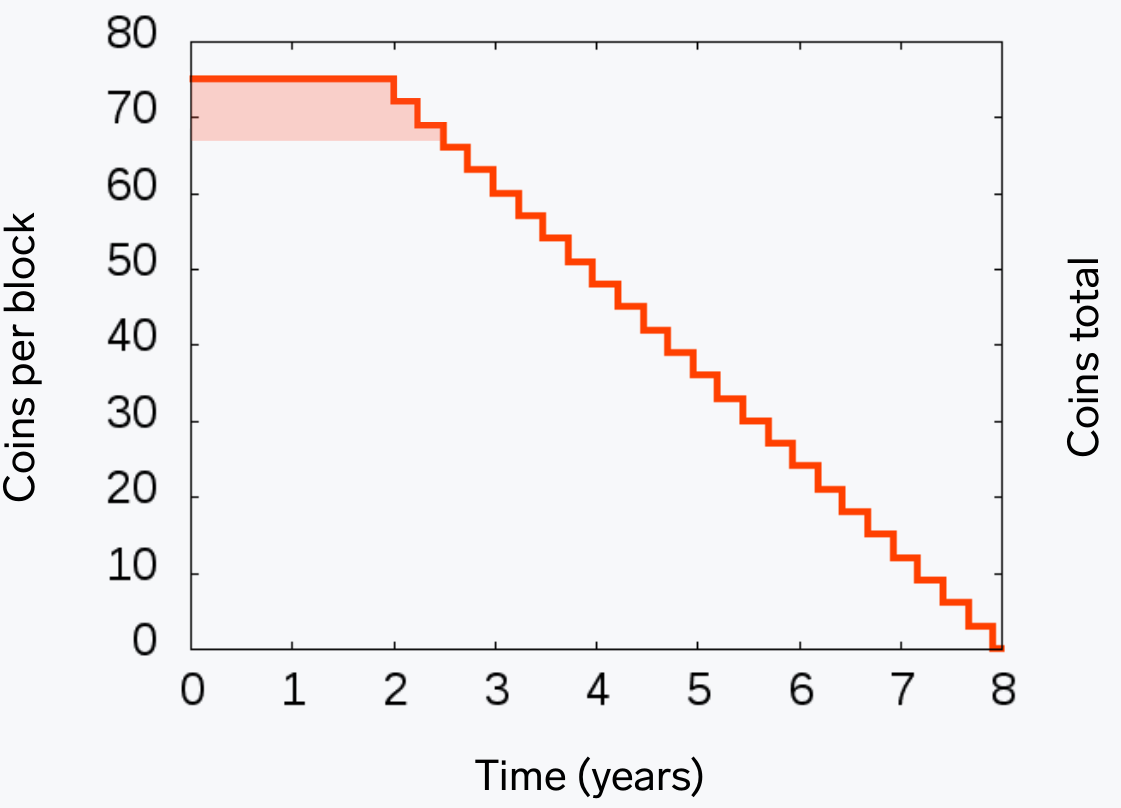
\includegraphics[width=\textwidth]{emission.png}
        \caption{Ergo emission curve
        \label{fig:emission} }
    \end{figure}


    \section{Applicability}

    To survive, a blockchain must have a user base.
    Light clients opens up opportunities for really decentralized applications and offchain protocols.
    However, they also require useful and safe smart contracts language.
    Ergo smart contracts are based on Bitcoin-like UTXO model, where every output is protected by some script.
    If scripting language is rich enough, it allows to write Turing-complete contracts~\cite{chepurnoy2018self}
    while avoiding ad-hoc solutions for program halting like gas in Ethereum.
    Ergo script only contains operations, that allow to estimate script complexity before execution,
    preventing various DoS attacks.
    However this instructions set is enough to easily write any possible program.
    Cryptographic part of Ergo script is based on sigma protocols and naturally supports
    threshold m-of-n signatures, ring signatures and more.


    \section{Conclusions}


    \bibliography{references}

\end{document}